\documentclass[10pt,a4paper]{article}
\usepackage[margin=18mm]{geometry}
\usepackage{graphicx}
\usepackage{booktabs}
\usepackage{tabularx}
\usepackage{array}
\usepackage{float}
\usepackage{caption}
\usepackage{subcaption}
\usepackage{xcolor}
\usepackage{hyperref}
\hypersetup{colorlinks=true, linkcolor=blue, urlcolor=blue}
\graphicspath{{figures/}}
\setlength{\parindent}{0pt}
\setlength{\parskip}{0.55em}

\title{DAMH ERT20 Free-$t_0$ Global-Archie Run Report}
\author{Generated from saved run artifacts}
\date{2026-06-15}

\begin{document}
\maketitle

\section*{Verdict}

This run is a \textbf{failed sampler run with useful pre-crash exact OGS diagnostics}.
The requested parametrisation was active: ERT $t_0$ was free, Archie parameters were fitted globally,
and the open-niche boundary parameters were fixed. The run did not reach the planned stop at
\texttt{2026-06-15 08:30 CEST}. The launcher exited at \texttt{2026-06-14 22:59:45 CEST}
with exit code \texttt{139}.

The immediate Python error was:
\begin{verbatim}
ValueError: cannot reshape array of size 640 into shape (20,33)
\end{verbatim}

The failed evaluation appears to be \texttt{solver14\_eval000003}. OGS itself finished with
return code 0, but post-processing returned 640 ERT values, i.e. $20 \times 32$, while the
likelihood expected 660 values, i.e. $20 \times 33$.

\section*{Configuration}

\begin{tabularx}{\linewidth}{@{}lX@{}}
\toprule
Campaign & \texttt{damh\_ert20\_t0\_free\_global\_archie\_su\_until\_20260615\_0830\_v1} \\
Feature count & 208 \\
Observation count expected by likelihood & 660 \\
MPI size & 16 \\
Archie mode & \texttt{global} \\
Free ERT $t_0$ & \texttt{True} \\
$t_0$ prior & mean 96.081672 d, std 10.00 d, bounds [66.081672, 106.081672] d \\
Open-niche boundary & fixed: shift 0.0 d, suction scale 1.0, suction offset 0.0 MPa \\
Dataset & \texttt{dataset\_arrays.npz} from \texttt{ert20\_t0\_free\_global\_archie\_current} \\
Warm checkpoint & \texttt{ert20\_theta\_mlp\_warm.pt} from \texttt{ert20\_damh\_t0\_free\_global\_archie\_seed} \\
\bottomrule
\end{tabularx}

\section*{Run Outcome}

\begin{tabular}{@{}lr@{}}
\toprule
Metric & Value \\
\midrule
Result manifest written & \texttt{2026-06-14T22:45:32+02:00} \\
First exact candidate summary & \texttt{2026-06-14T22:49:51+02:00} \\
Last exact candidate summary & \texttt{2026-06-14T22:59:38+02:00} \\
Launcher exit code & \texttt{139} \\
Exact candidate summaries & 44 \\
Candidate status counts & \texttt{\{'evaluated': 44\}} \\
Likelihood history rows & 4140 \\
Likelihood calls & 207 \\
Likelihood history modes & \texttt{\{'global': 4140\}} \\
surrDAMH raw/sample/accepted rows flushed & 1 / 1 / 1 \\
\bottomrule
\end{tabular}

Because only one surrDAMH sampling row was flushed, this run does \textbf{not} provide a
meaningful posterior trace, accepted-sample ensemble, or convergence diagnostic. The reliable
data products are the 44 exact OGS candidate summaries and their residual, Archie, and theta files.

\begin{figure}[H]
\centering
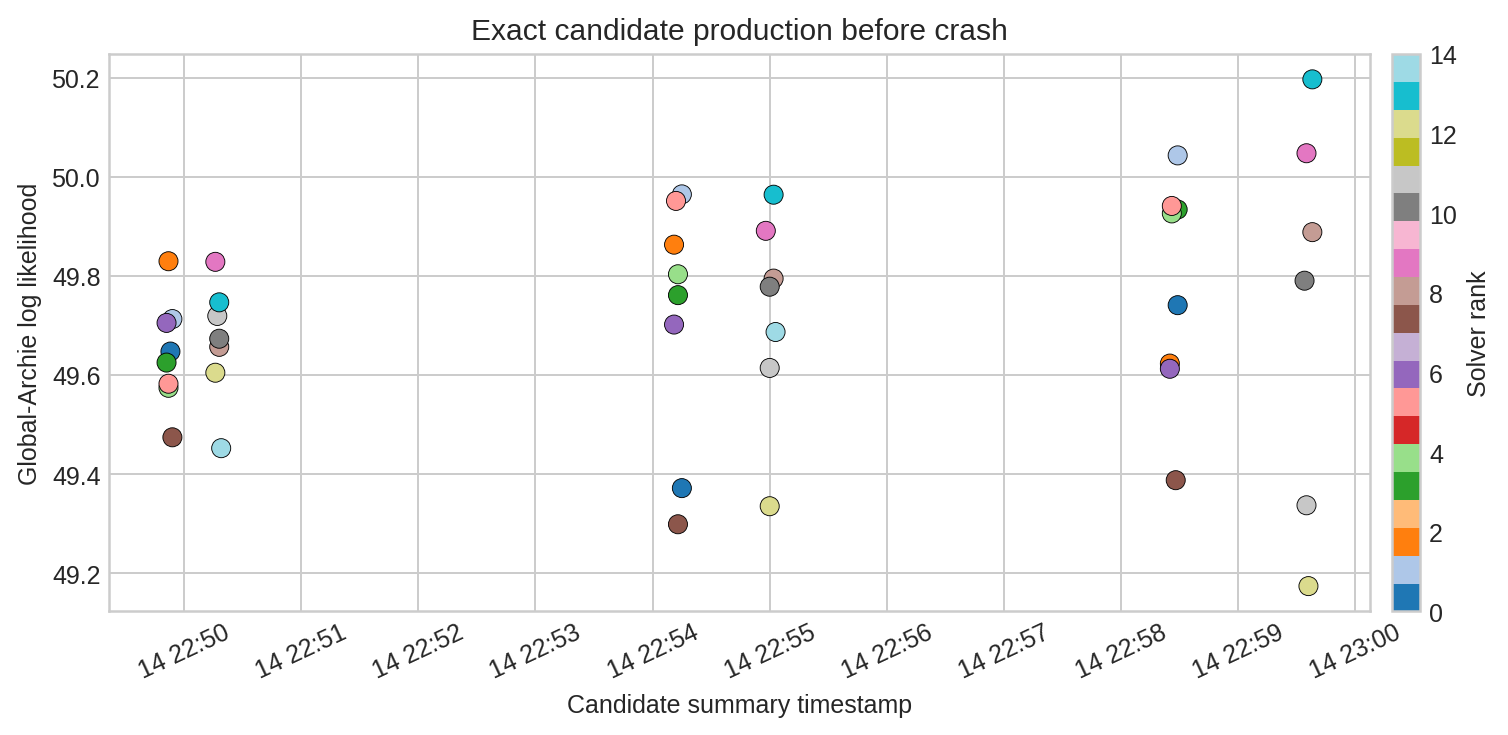
\includegraphics[width=0.92\linewidth]{01_candidate_timeline_likelihood.png}
\caption{Exact-candidate production before the crash.}
\end{figure}

\section*{Exact Candidate Diagnostics}

All summarized exact candidates used \texttt{archie\_mode = global}, had
\texttt{theta\_output\_count = 660}, and kept fixed open-niche boundary values.

\begin{tabular}{@{}lrrrr@{}}
\toprule
Quantity & Min & Median & Mean & Max \\
\midrule
Local Archie log likelihood & 49.1736 & 49.7161 & 49.7104 & 50.1971 \\
Local Archie MAE & 0.08243 & 0.08368 & 0.08376 & 0.08546 \\
Local Archie objective & 0.33679 & 0.34882 & 0.34896 & 0.36238 \\
Global Archie $\log_{10}(a)$ & 1.05834 & 1.07766 & 1.07875 & 1.11161 \\
Global Archie exponent $b$ & -0.48113 & -0.46530 & -0.46284 & -0.42675 \\
ERT $t_0$ shift [days] & 89.6880 & 95.4619 & 95.4769 & 100.3196 \\
$k_0$ $\log_{10}(k\,m^2)$ & -21.2935 & -20.9788 & -20.9960 & -20.5290 \\
Homogeneous porosity & 0.14018 & 0.14854 & 0.14798 & 0.15305 \\
Bedding angle [deg] & 138.7395 & 139.4510 & 139.4174 & 140.0752 \\
$q_{22}/q_{11}$ & 0.43484 & 0.44953 & 0.45104 & 0.47322 \\
\bottomrule
\end{tabular}

\begin{figure}[H]
\centering
\begin{subfigure}{0.48\linewidth}
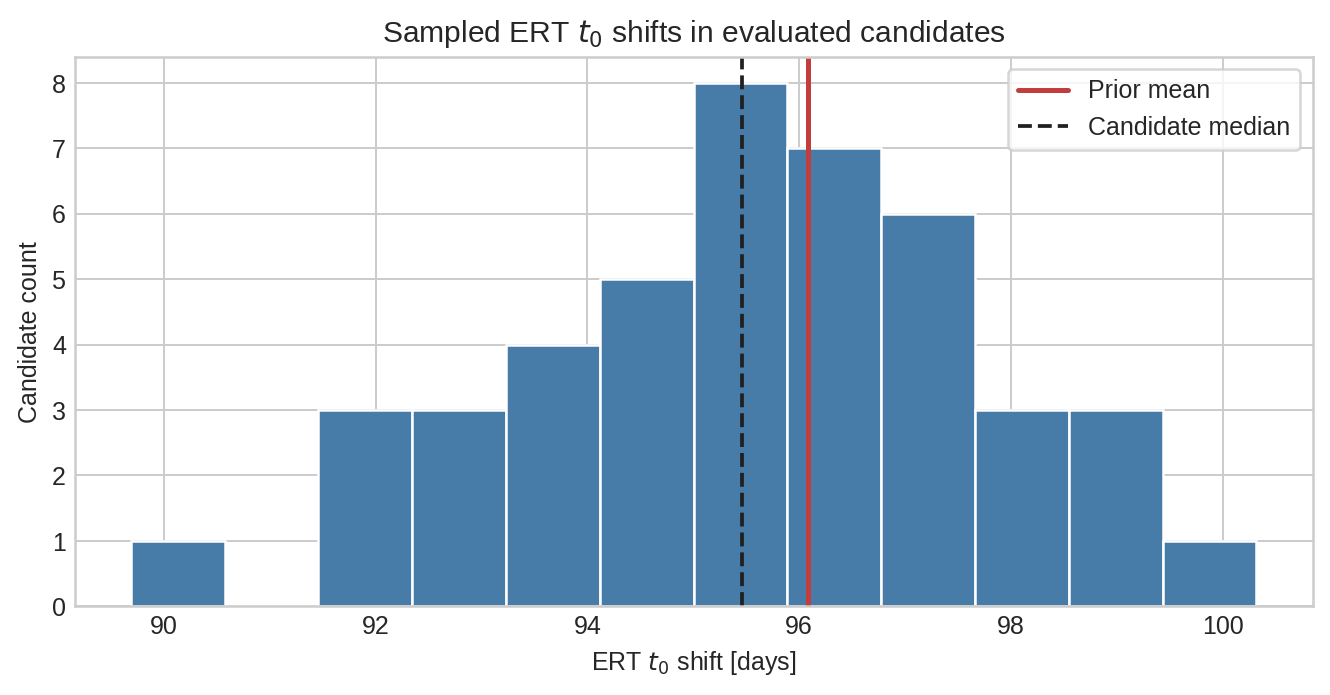
\includegraphics[width=\linewidth]{02_t0_shift_distribution.png}
\caption{$t_0$ shift distribution.}
\end{subfigure}\hfill
\begin{subfigure}{0.48\linewidth}
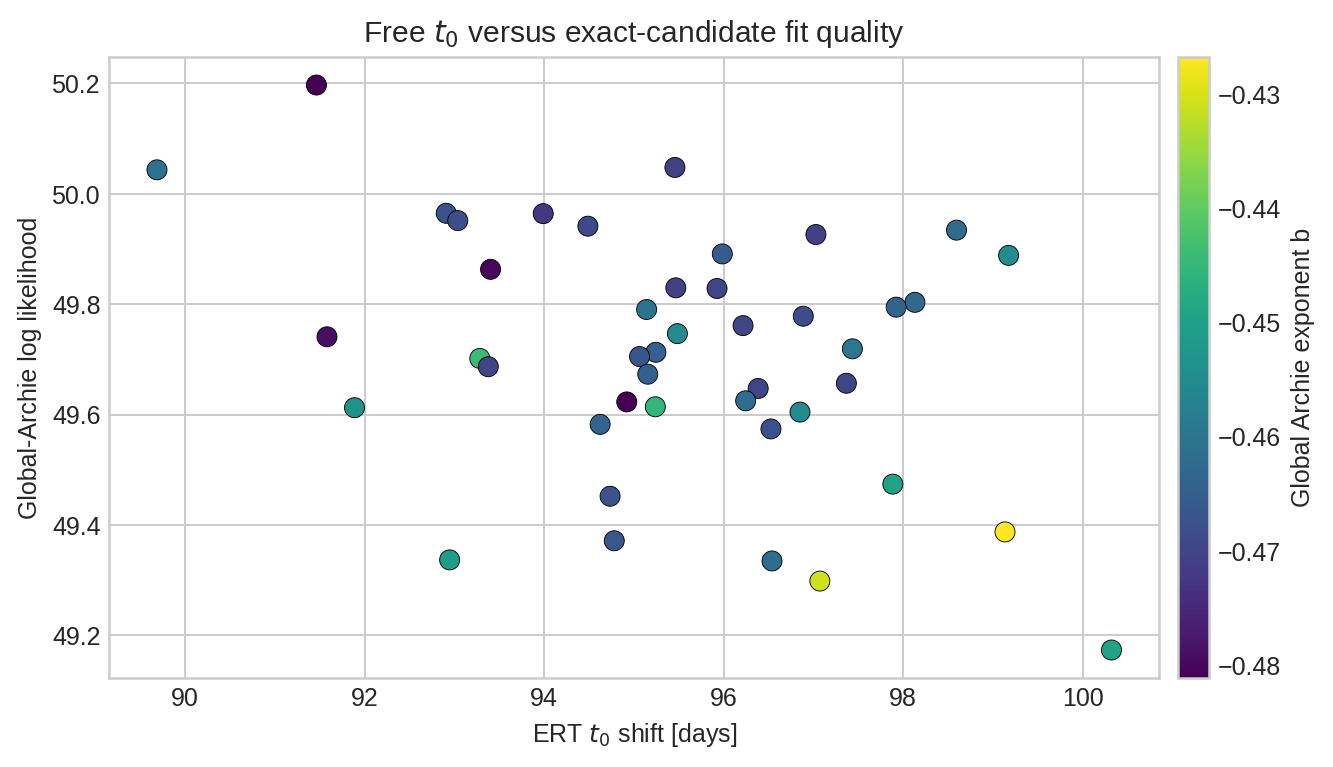
\includegraphics[width=\linewidth]{03_t0_vs_likelihood.png}
\caption{$t_0$ shift versus fit quality.}
\end{subfigure}
\caption{The free ERT $t_0$ shift was active in the valid candidates.}
\end{figure}

\begin{figure}[H]
\centering
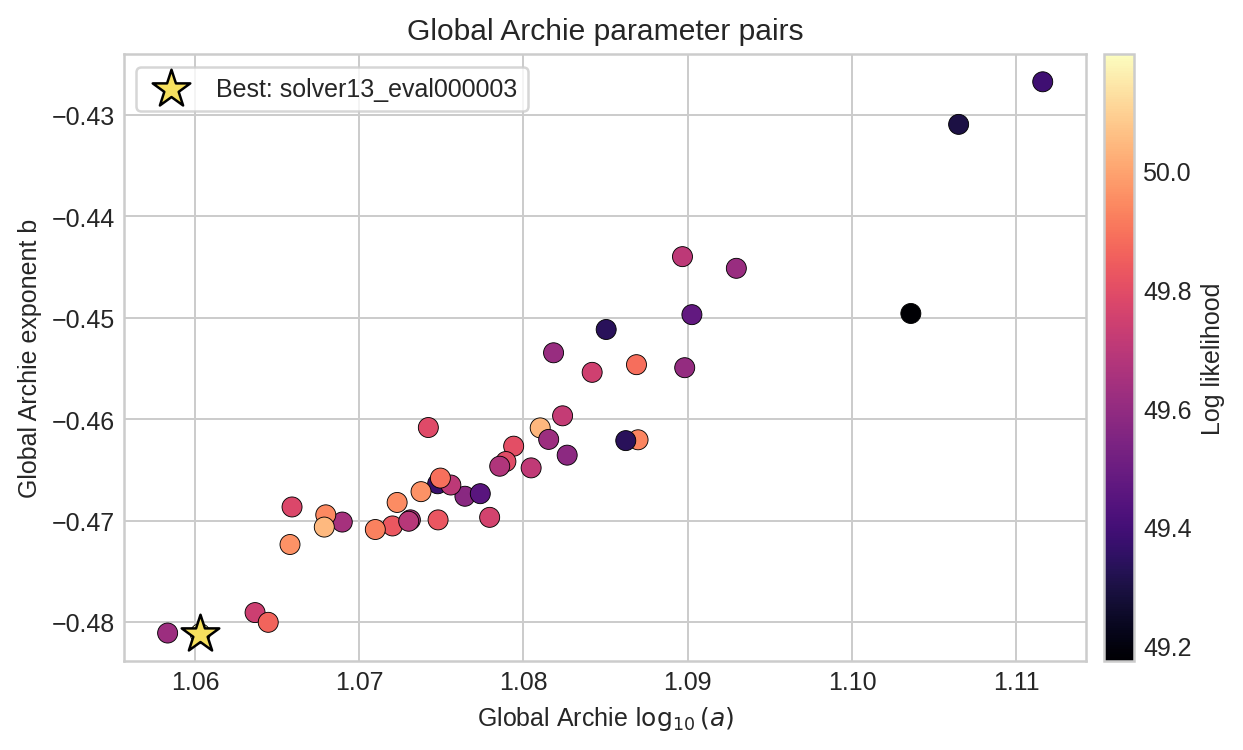
\includegraphics[width=0.72\linewidth]{04_global_archie_pairs.png}
\caption{Global Archie parameter pairs fitted for each exact candidate.}
\end{figure}

\section*{Top Exact Candidates}

Best exact candidate by global-Archie likelihood: \texttt{solver13\_eval000003}.

\begin{tabular}{@{}rlrrrrr@{}}
\toprule
Rank & Candidate & Log likelihood & MAE & $t_0$ shift [d] & Global $\log_{10}(a)$ & Global $b$ \\
\midrule
1 & \texttt{solver13\_eval000003} & 50.197105 & 0.082541 & 91.463850 & 1.060321 & -0.481130 \\
2 & \texttt{solver09\_eval000003} & 50.047850 & 0.082492 & 95.456776 & 1.067875 & -0.470627 \\
3 & \texttt{solver01\_eval000003} & 50.043519 & 0.083309 & 89.687973 & 1.081020 & -0.460855 \\
4 & \texttt{solver01\_eval000002} & 49.964777 & 0.083288 & 92.909363 & 1.073765 & -0.467137 \\
5 & \texttt{solver13\_eval000002} & 49.964145 & 0.082861 & 93.989998 & 1.065788 & -0.472344 \\
\bottomrule
\end{tabular}

\begin{figure}[H]
\centering
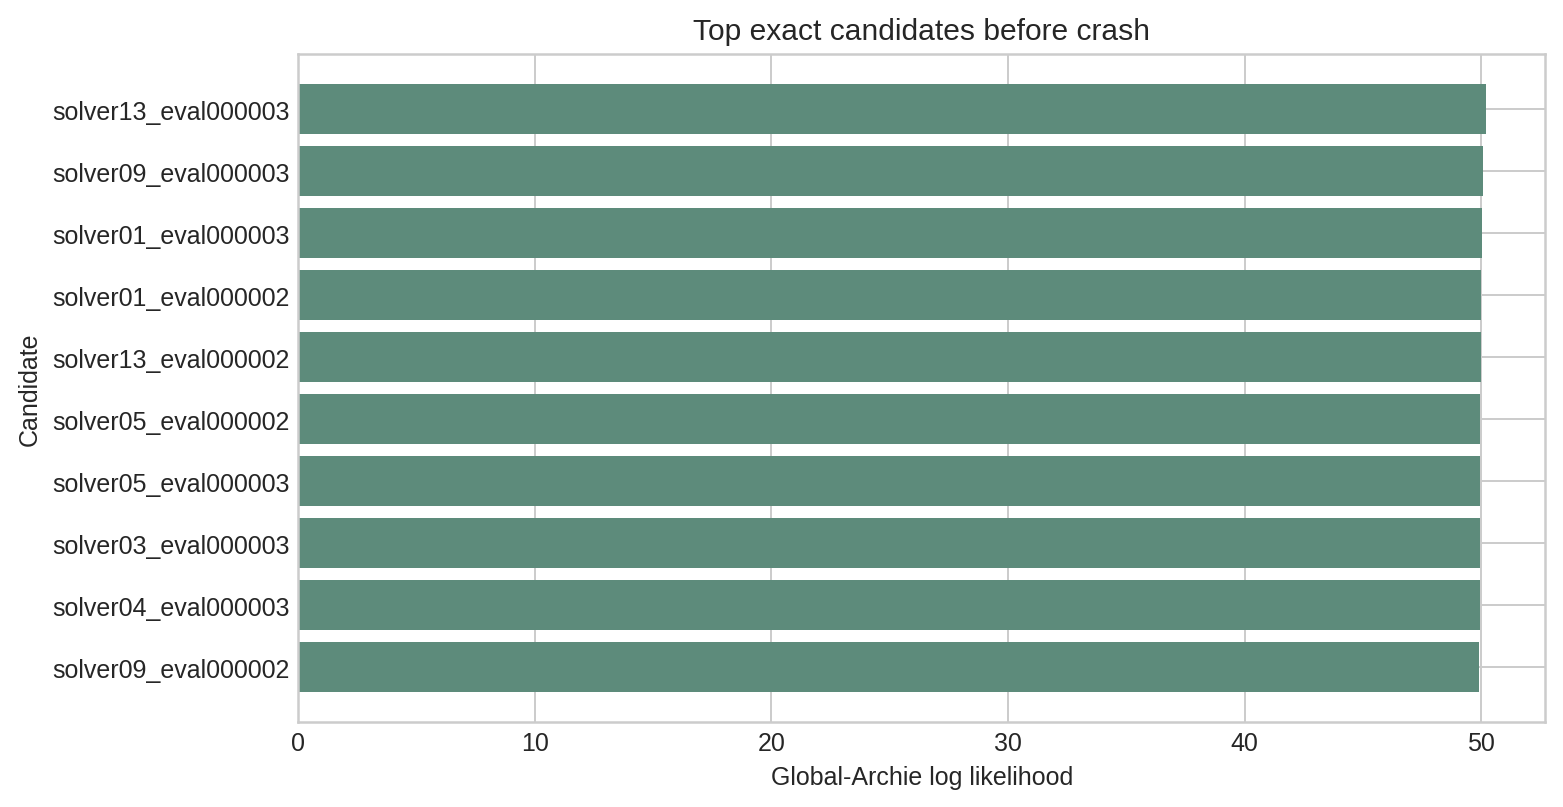
\includegraphics[width=0.80\linewidth]{08_top_candidates.png}
\caption{Top ten evaluated exact candidates before the crash.}
\end{figure}

\section*{Best Candidate Residual Diagnostics}

\texttt{solver13\_eval000003} has log likelihood 50.197105,
MAE 0.082541, $t_0$ shift 91.463850 days,
global $\log_{10}(a)$ 1.060321, and global $b$
-0.481130.

\begin{figure}[H]
\centering
\begin{subfigure}{0.58\linewidth}
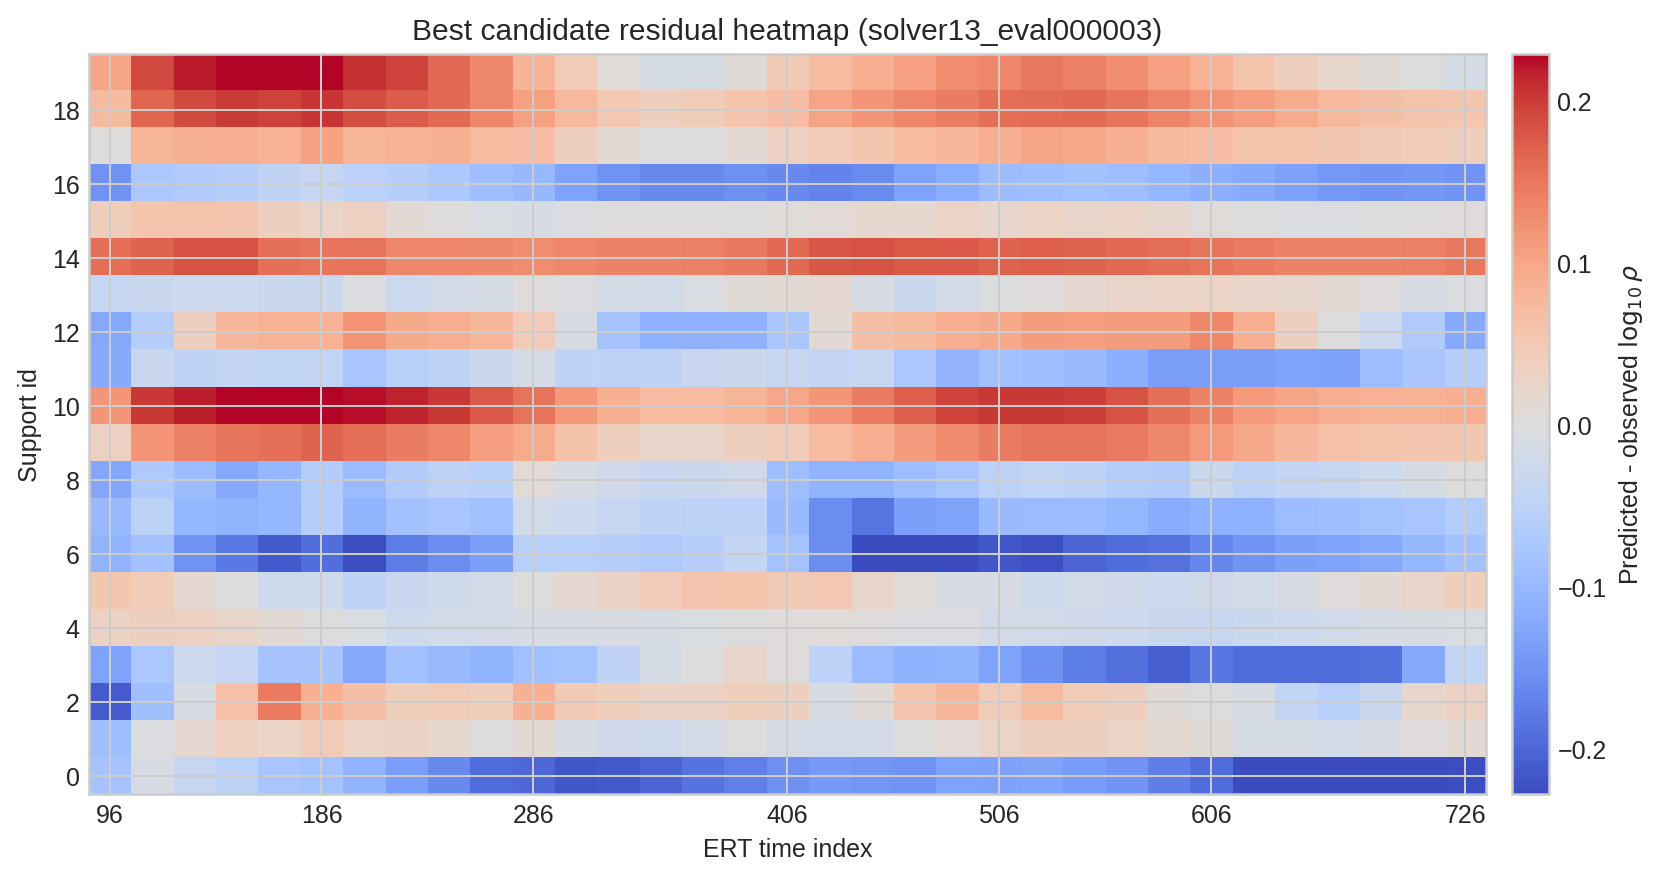
\includegraphics[width=\linewidth]{05_best_residual_heatmap.png}
\caption{Residual heatmap.}
\end{subfigure}\hfill
\begin{subfigure}{0.36\linewidth}
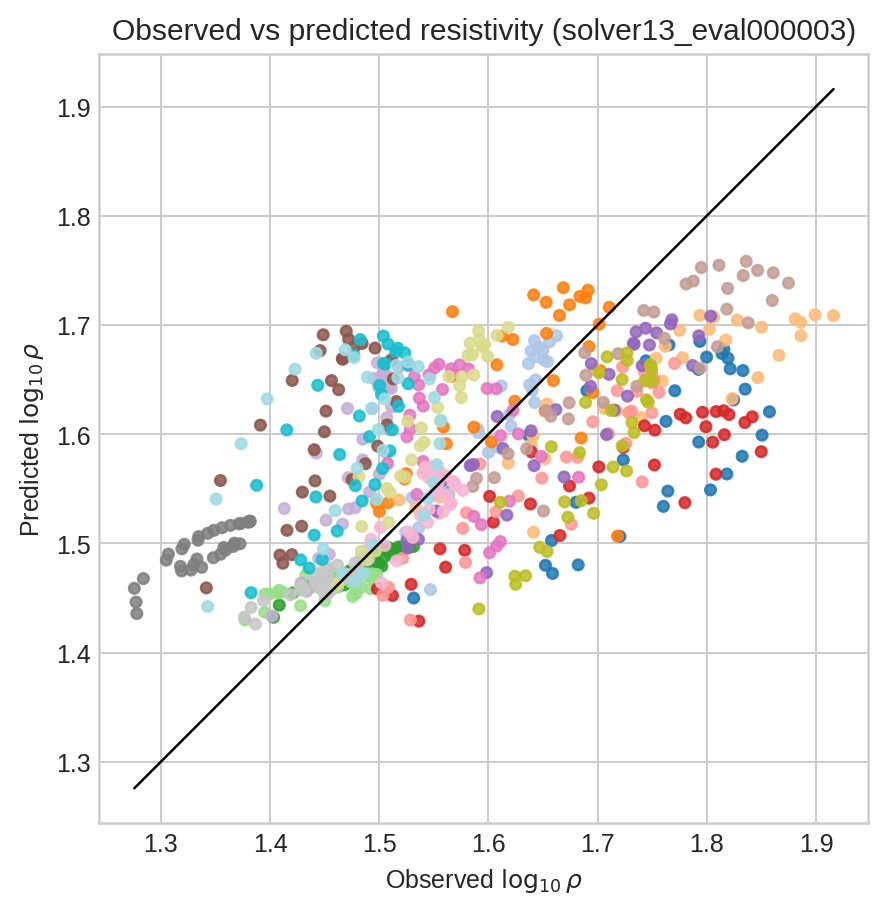
\includegraphics[width=\linewidth]{06_best_observed_vs_predicted.png}
\caption{Observed versus predicted.}
\end{subfigure}
\caption{Best-candidate ERT residual checks.}
\end{figure}

\begin{figure}[H]
\centering
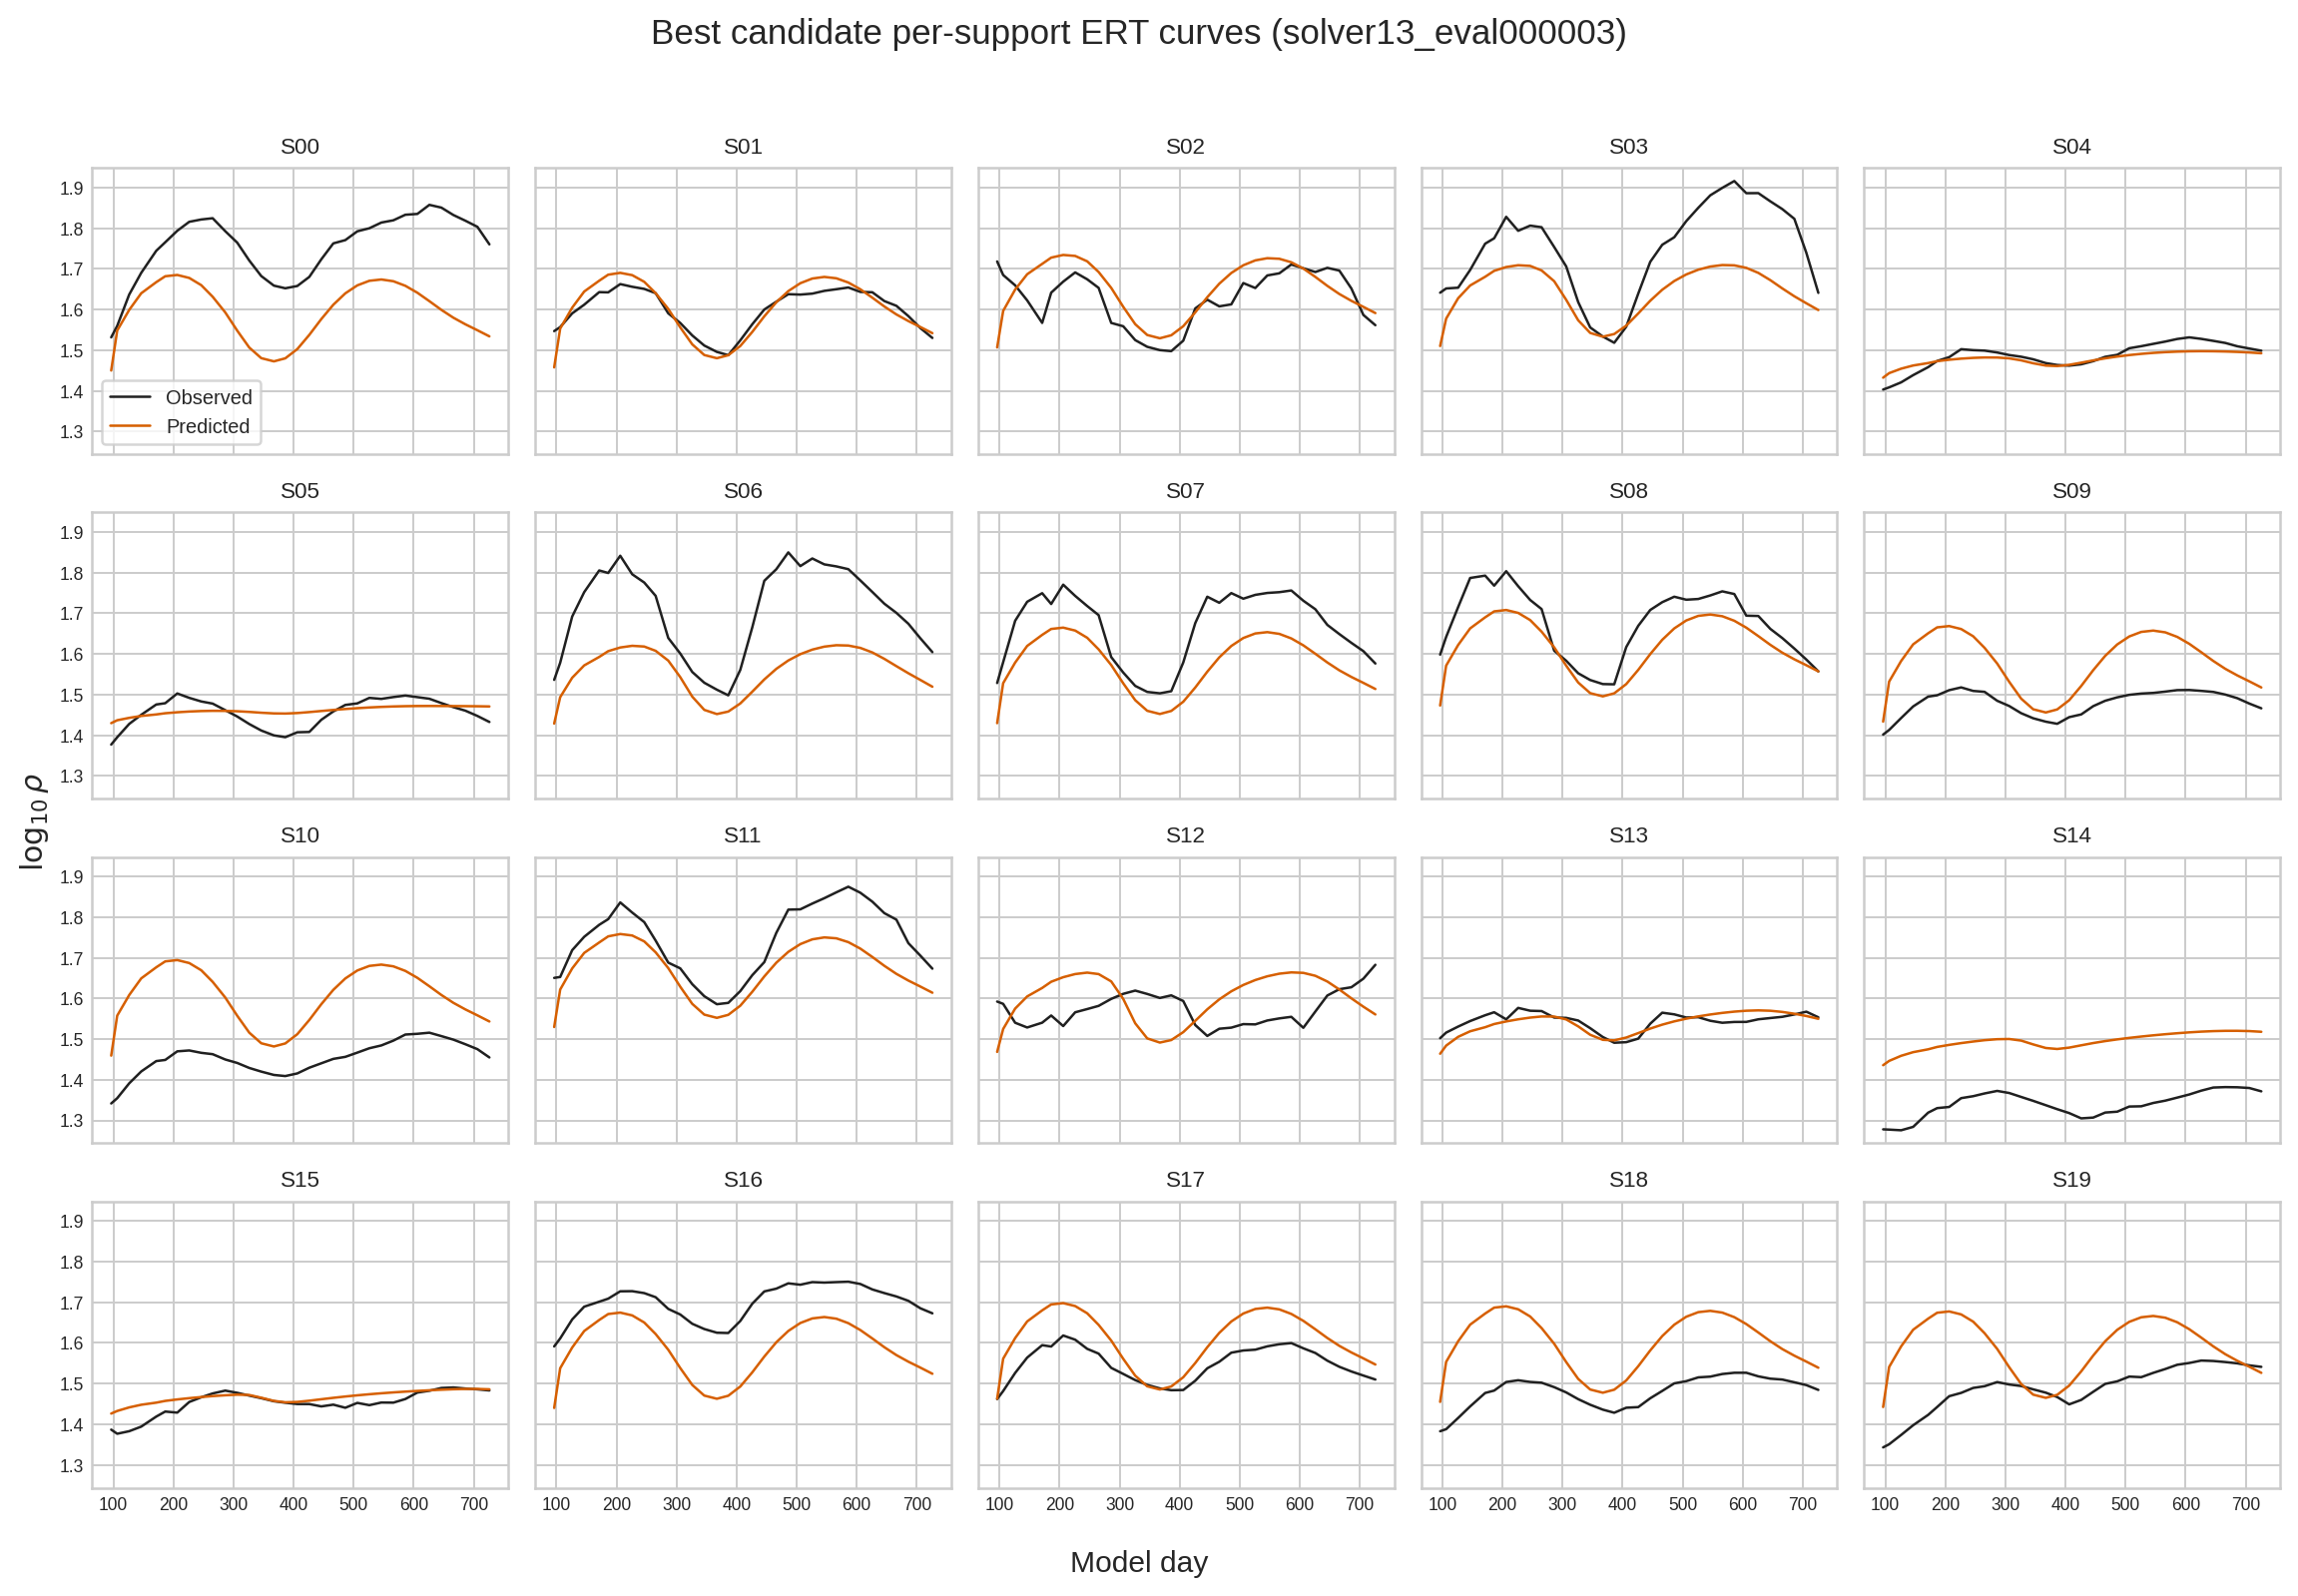
\includegraphics[width=\linewidth]{07_best_support_curves.png}
\caption{Observed and predicted ERT curves for all 20 supports for the best exact candidate.}
\end{figure}

\section*{Archie Spatial Comparison}

The previous fixed-boundary deep run fitted Archie parameters independently per support, while
this free-$t_0$ run fitted a single global Archie pair. The radial plot below uses support azimuth
as the polar angle and separates the two ERT support depths into two traces. The dashed rings show
the current best global Archie value.

\begin{figure}[H]
\centering
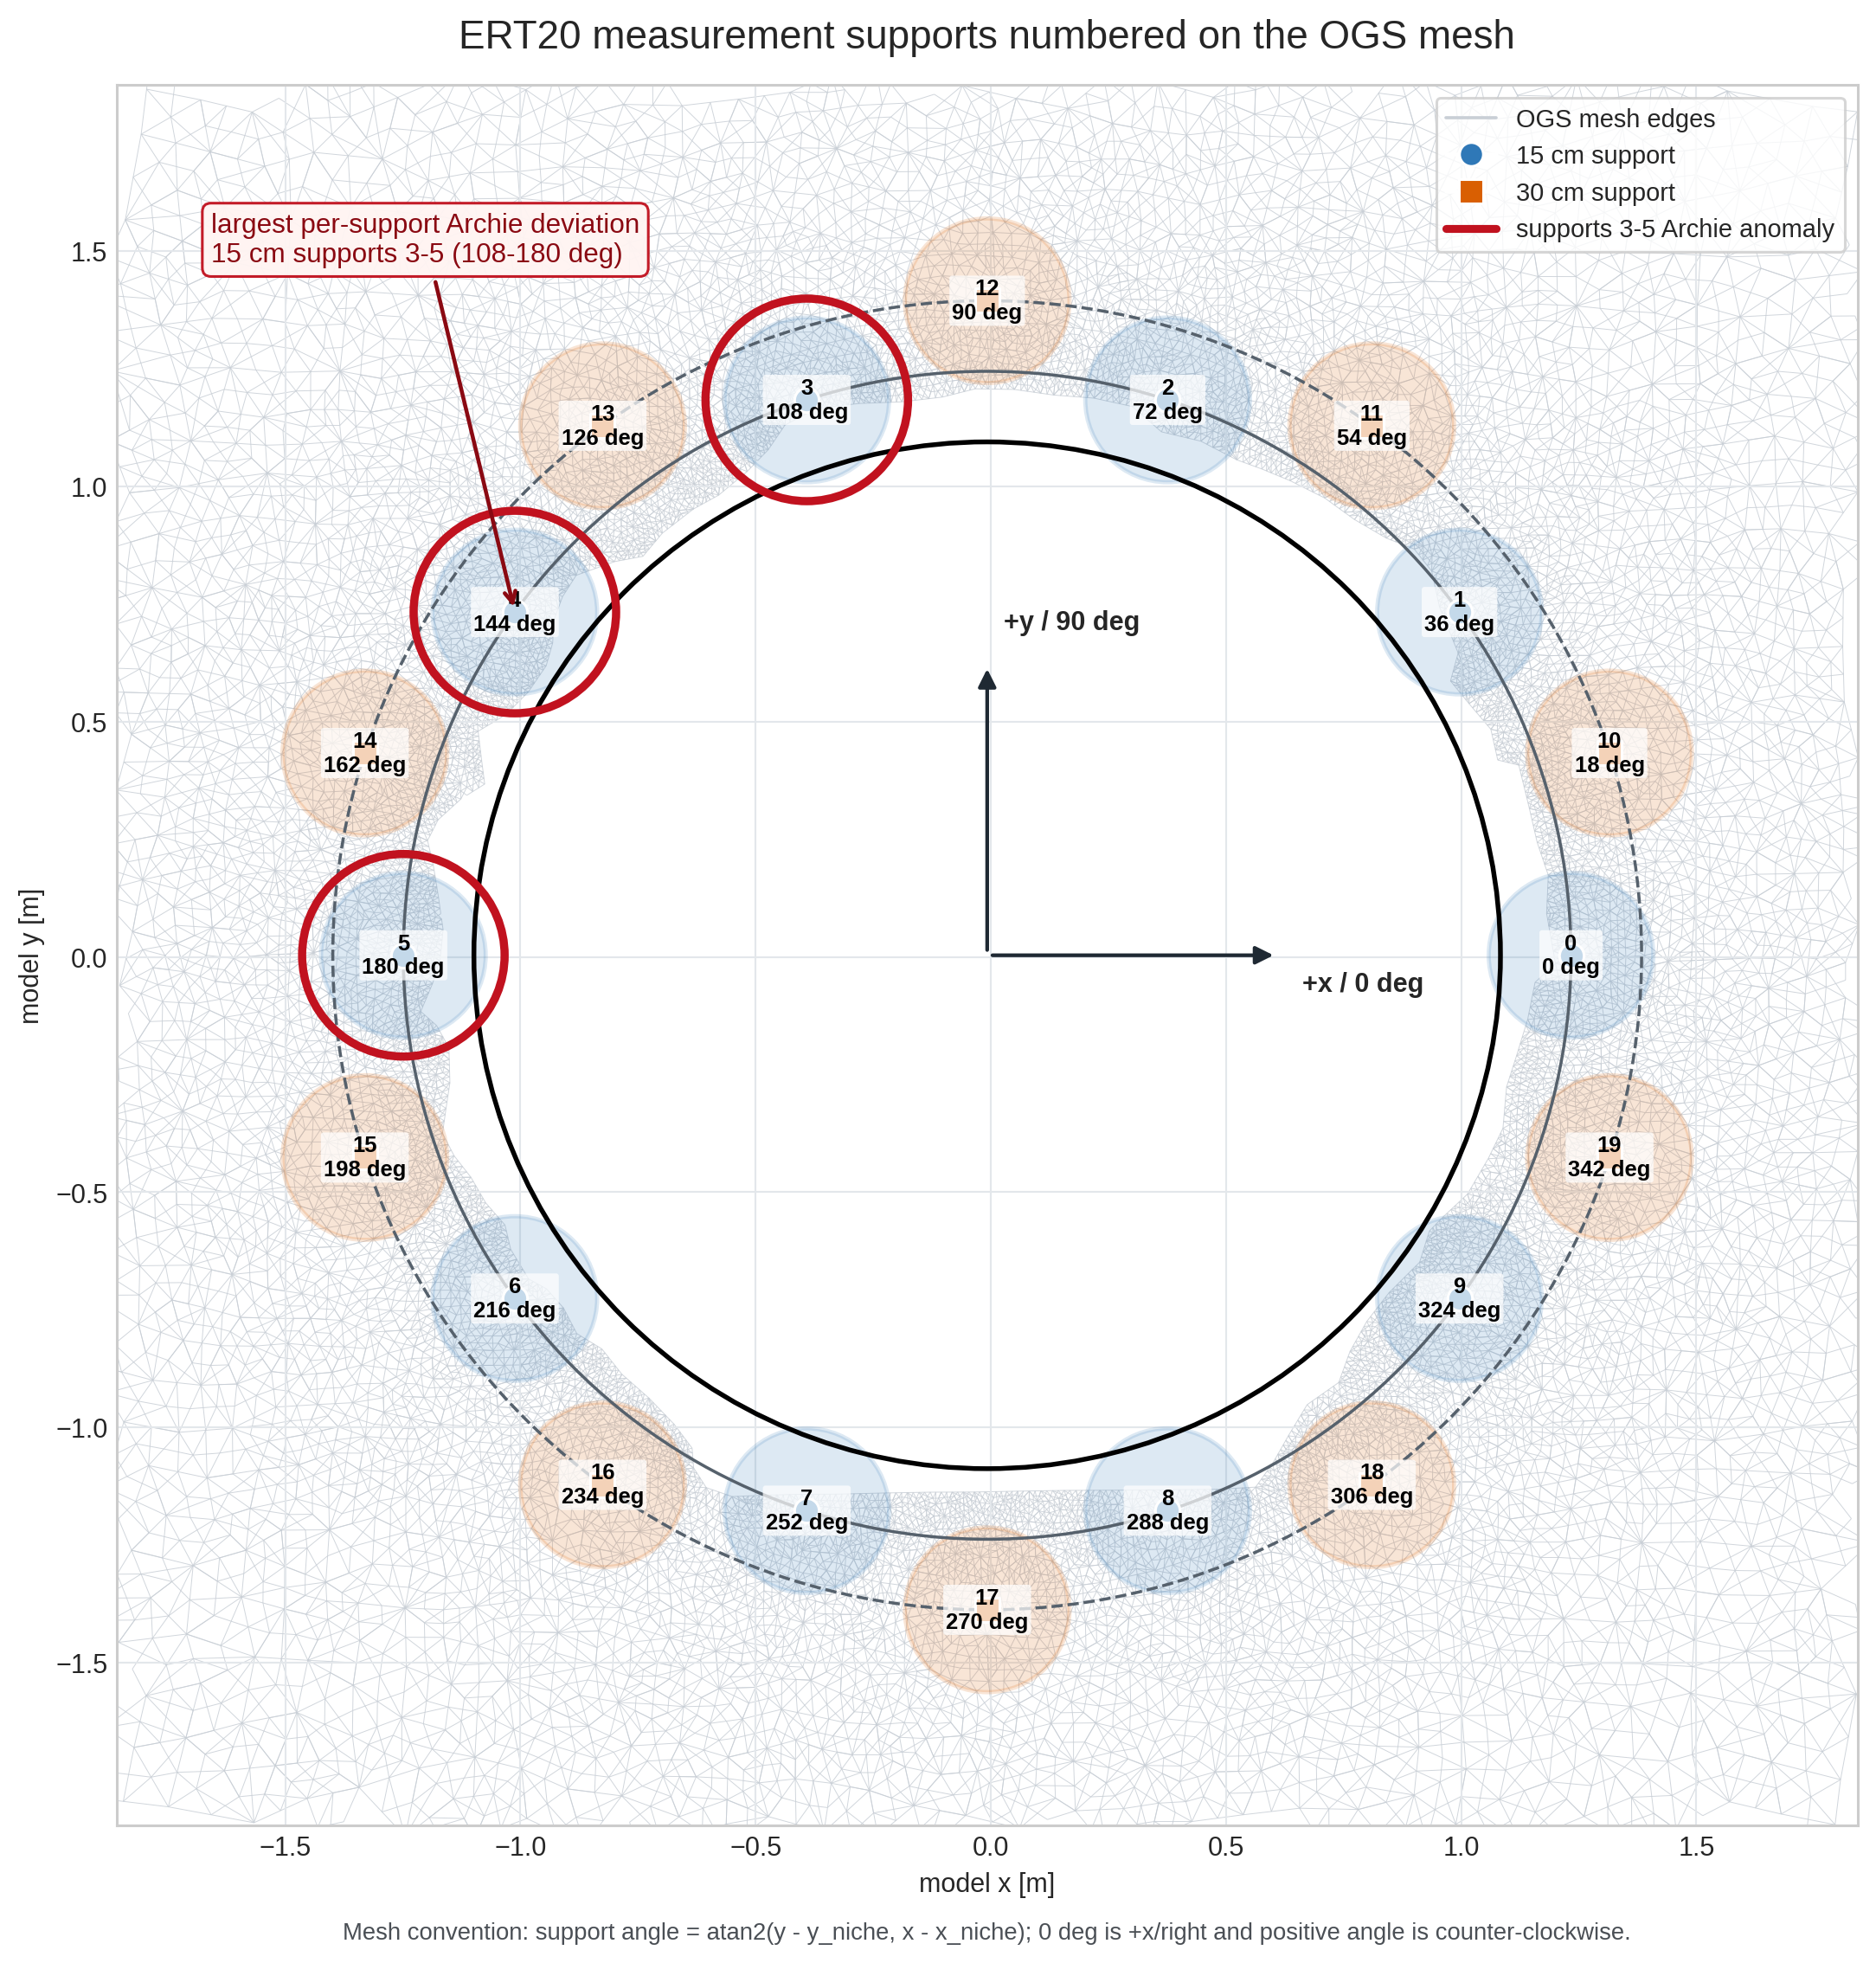
\includegraphics[width=0.92\linewidth]{11_ert20_supports_numbered_on_mesh.png}
\caption{ERT20 measurement supports numbered on the OGS mesh. The red halos mark supports 3--5, the shallow 15 cm locations with the strongest previous per-support Archie departure.}
\end{figure}

\begin{center}
\fcolorbox{red!65!black}{yellow!12}{%
\begin{minipage}{0.93\linewidth}
\textbf{Important spatial note for follow-up agents.}
The strongest departure from the global Archie pair is spatially localized and is dominated by
the shallower 15 cm support trace, especially supports 3--5 at 108--180 degrees in the previous
per-support fit. In the mesh-aligned coordinates this is the left/upper-left sector, not the
bottom of the page; if a field-view niche drawing is rotated, translate the feature by support
IDs/angles rather than by page position. A plausible hypothesis is that shallow/surface electrical
current paths, contact effects, or near-boundary current leakage are breaking the simple
OGS-theta-plus-Archie ERT model locally. This is not proven by the plot alone, but it is important
enough to test explicitly before interpreting the global-Archie failure as a purely hydraulic or
porosity-field problem.
\end{minipage}}
\end{center}

\begin{figure}[H]
\centering
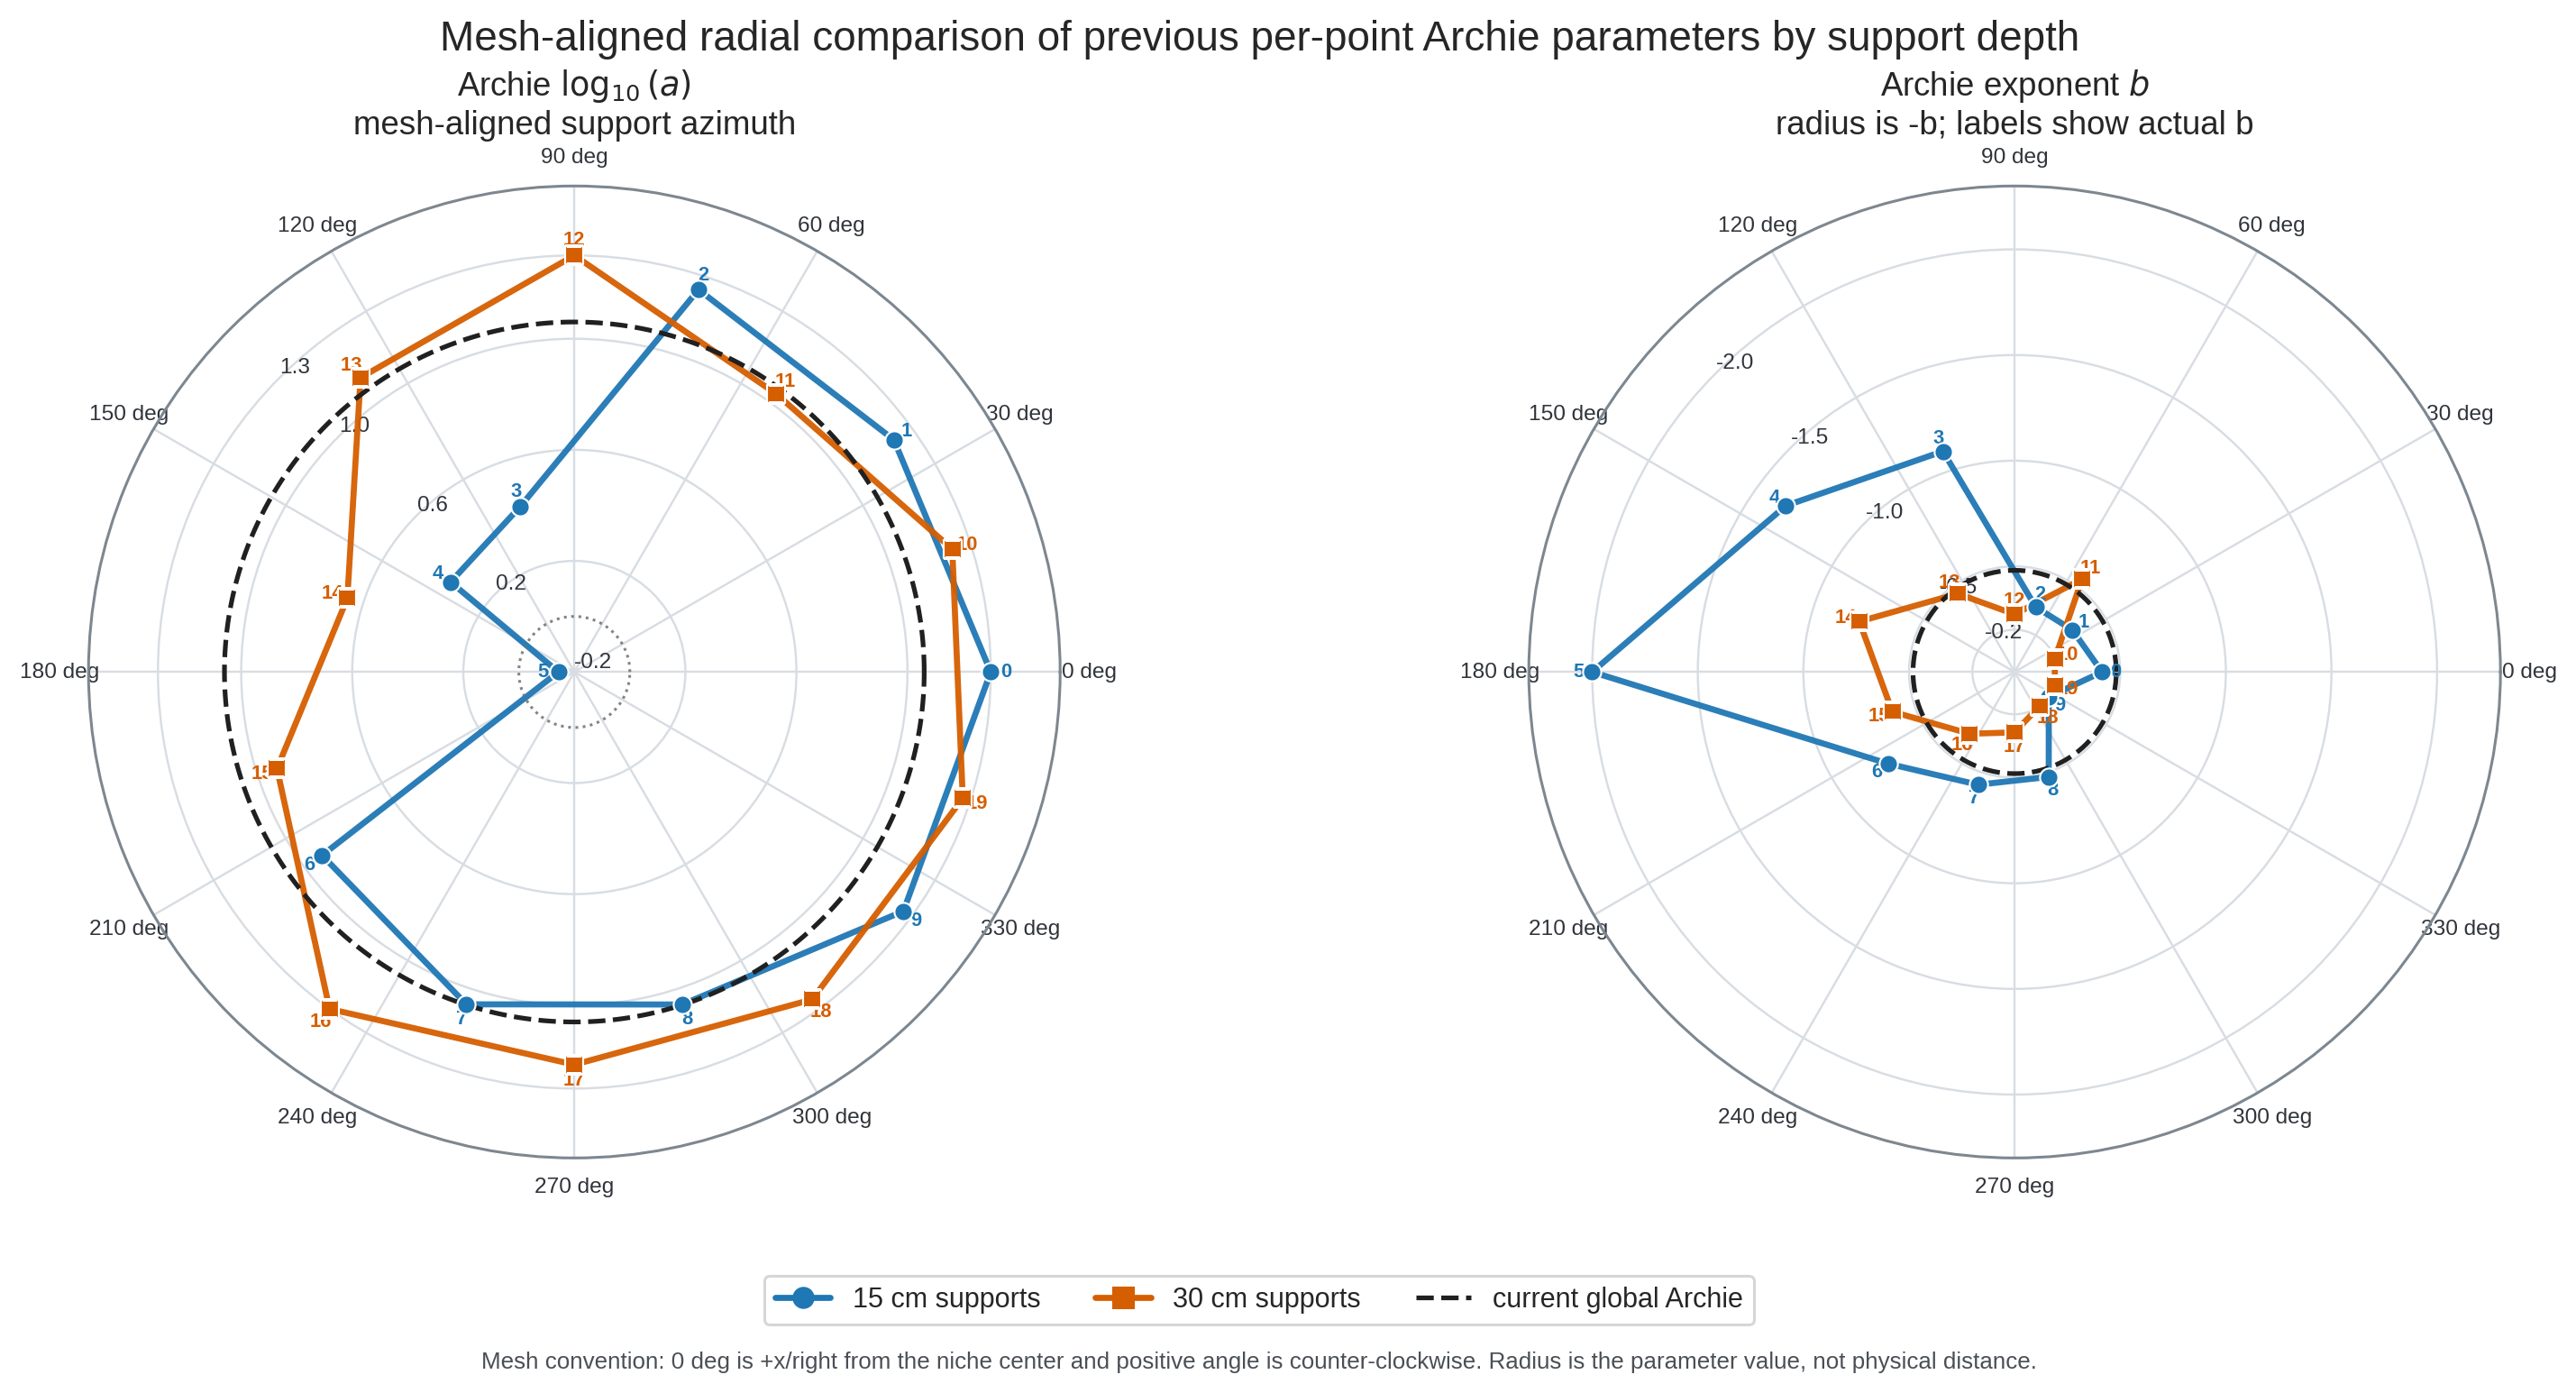
\includegraphics[width=\linewidth]{10_archie_radial_by_depth.png}
\caption{Mesh-aligned radial comparison of previous per-support Archie parameters against the current global Archie reference. The polar angle follows the support-table convention: $0^\circ$ is positive mesh $x$ from the niche center and angles increase counter-clockwise.}
\end{figure}

\section*{Failure Analysis}

The core failure was a solver/likelihood contract mismatch:
\[
\mathrm{expected} = 20 \times 33 = 660,\qquad
\mathrm{actual} = 20 \times 32 = 640.
\]

Since the failed OGS run completed successfully, the likely failure surface is the
ERT extraction and time-alignment step after OGS. A free $t_0$ perturbation can move one ERT
measurement time outside the matched OGS output-time window, or outside the matching tolerance,
leaving only 32 matched time points. The likelihood then attempted to reshape the vector into the
fixed observed-data shape and crashed.

\section*{Scientific Use}

\textbf{Usable:} the 44 evaluated exact candidate summaries; confirmation that free $t_0$ was
sampled; confirmation that global Archie fitting was active; confirmation that the fixed
open-niche boundary stayed fixed; rough early diagnostic distributions for fit quality and scalar
parameters.

\textbf{Not usable:} posterior samples, acceptance-rate diagnostics, long-run convergence
diagnostics, final surrogate-updated ensemble, or any morning-completion claim.

\section*{Recommended Relaunch Fix}

Before relaunching, enforce that every candidate returns exactly $20 \times 33 = 660$ ERT values.
If a shifted ERT date cannot be matched, either interpolate to the nearest valid OGS interval or
reject the candidate with $-\infty$ likelihood before calling the Archie likelihood. Also add an
explicit size guard in \texttt{get\_observations} so one malformed candidate writes a failure
summary instead of taking down MPI.

\end{document}
